\section{Introduction}

The increase in informal housing is a common issue faced by nations globally.
Although informal regions of housing, such as slums, are commonplace in
underdeveloped countries, it affects the developed world as well, e.g., refugee
camps. Informal settlements might be difficult to monitor merely on the usage
of ground surveys due to scale, distribution or a varity of other difficulties.
Satellite and aerial images provide a solution to the problems encountered with
ground based methods.  High resolution images allow for the detection of
informal housing based exclusively on features extracted from the image.  The
images could be annotated manually although the feasability diminishes with
increased scale.  As a solution, the detection of informal settlements can be
automated using inherent visual characteristics of a certain area. The features
extracted images provide a distinct difference between formal and informal
housing. The features that are determined distinctive can used by classification
algorithms, effectively automizing the detection of areas containing informal
housing in images.

\subsection{Global Context}
% state
According Un-Habitat, close to a third of the global urban population lives in informal settlements \cite{2016state}. In specific parts of the world, for instance Sub-Saharan Africa, the urban population that lives in informal housing is estimated to be close to two thirds of the total urban population \cite{un2013planning}. In the past decades, the percentage of slum inhabitants compared to the urban population has decreased. Paradoxically, in absolute terms, the total number has actually increased \cite{2016state}.

% definition and negative effects
Informal settlements exist globally, although often in different forms and described using different names. The individuals living in informal settlements, such as slum dwellers, are specified by Un-Habitat by one ore more of the following conditions: inadequate  drinking  water,  inadequate  sanitation, poor  structural quality of housing, over crowding and insecurity of tenure \cite{un2015slum}. In addition, the inhabitants of slums experience social and economical exclusion from the opportunities that an urban environment offers. Furthermore, slum dwellers are prone to natural disasters in addition to disease outbreaks. 

% solution
Over the years, there have been multiple governmental policies implemented to address the problem of informal settlements. Informal settlements were largely tolerated and neglected, large eviction and resettlement of the inhabitants were not found to be effective \cite{kuffer2016slums}. Instead, in recent years, a less intrusive approach is used in solving the slum problem. This method enables governments to solve the slum question by supporting the upgrade of slums to formal housing \cite{cobbett2013cities}. Besides government policy, Un-Habitat allocates a significant effort to the use of this method itself\cite{2015globact}.

\subsection{Related works and contributions}
% into remote sensing
In many cities in the developing world, slums are a large part of the urban environment. However, there is often a lack of information about the properties of the slum, such as the location, the scale and the population \cite{kuffer2016slums}. These cities often do not have the resources to obtain this information. Remote sensing is able to provide the often lacking  socialeconomic information. Besides, remote sensing is also able to capture the spatial and temporal dynamics of the informal areas, which supports urban planning and the development of the city.

% methods
In the last decade, access to satellite images was becoming widespread along side an increase in methods for urban area classification \cite{kuffer2016slums}. This allowed for informal areas to be studied throughout the globe, e.g. Colombo \cite{colombo}, Johannesburg \cite{williams2016automatic}, Accra \cite{accra}, Mumbai \cite{mumbai}, Rio de Janeiro \cite{hofmann2008detecting}, and Hyderabad \cite{hyderabad}. With the increase interest in slum detection, it became apparent that the structural characteristics of slums were quite different from formal areas. This led to a large number of approaches based on the extraction of  image based features from satellite images. These approaches are, among others: the presence of vegetation \cite{niebergall2007object}, the size and shapes of buildings \cite{hofmann2008detecting}, the roofing material \cite{williams2016automatic}, texture features \cite{mattia2007exploiting}, and road accesability \cite{owen2013approach}.

Currently, the majority of studies uses the pixel image data of informal regions to extract features \cite{kuffer2016slums}. A different approach would be the characterization of areas by the objects that inhabit them. This is, for example, the detection of individual roofs in a certain area  of an image \cite{williams2016automatic}. Another example of this object based approach is the detection of road systems to characterize image regions. Alternatively, studies have used land use information \cite{novack2010urban} or social economical statistics \cite{engstrom2011using} to detect informal settlements.

% results
% The performance of the methods used in the studies is very variable. There are studies that have achieved a very high accuracy of in the 90\%. 

% conclusion prev work
%Because slums vary incredibly between different cities and regions, it is hard to obtain consensus about characteristics that well define informal areas. This variety makes it hard to create a method that will capture all the types of informal areas. As a result, the results obtained by the studies are quite specific to the studied city or area. 

 
\subsection{Proposed Method}

Our thesis continues with the work performed by Graesser \textit{et al.} \cite{graesser2012image}.
The paper characterized formal and informal neighborhoods using a set of different
features extracted from satellite images. Their approach was able to successfully characterize the
two types of neighborhoods with high accuracy on certain parts of the urban landscape. We will evaluate two of the feature extraction methods described in the paper from Graesser \textit{et al.} and attempt to reproduce similar results with satellite images from Bangalore. These methods are the Histogram of Oriented Gradients and Line support regions. Beyond the replication and evaluation of previous research, the methods of feature extraction used by Graesser \textit{et al.} will be extended by an additional new method.
This method creates a feature based on the density of road intersections in an image. The feature created from this method will be compared to the existing features and measured for its performance. The features produced by the three methods will combined and used by a set of different classification methods.
We will evaluate the different classification methods to discover the most suitable classification method for our image and its features. 

\subsection{Terminology}
% TODO: Move this somewhere else
% and rewrite bits
The paper of Graesser \textit{et al.} \cite{graesser2012image} uses blocks of pixels instead of each
individual pixel when extracting features from images.  This is to ease the
computational load because several of the extraction methods used are
computationally quite expensive. These blocks of pixels are of 20 by
20 pixels in the paper. The size of these pixel blocks will from this part on
be refered to as the \textit{block size}. The block size will differ from
this value to evaluate the affect to the performance of the features.
In addition to blocks, the paper also uses a set of different scales for the
calculation of features. A scale specifies the pixels around a block that
are used for the calculation of that block. This allows blocks to be more
spatially connected to the surrounding areas, which can increase the
performance of a feature.

\subsection{Data and Area of Study}
The image data used for the thesis is displayed in Figure \ref{fig:sections}d. The image has a resolution of 52,322 by 31,789 pixels with a filesize of 6.19GiB.
The image data is captured in 2012 by the earth observation satellite WorldView3 owned by DigitalGlobe. The WorldView3 satellite produces multiple types of images
with varying degrees of resolution. The panchromatic images have a resolution
of 0.31 meter in contrast to  the multiband images have a significantly lower
resolution of 1.24 meter. The project uses pansharpened images, which combines
the high resolution panchromatic- and the low resolution multiband images to
create high resolution RGB images.

The content of the images contain an area on the west of Bangalore, which is the capital city of the Indian state of Karnataka, located in south central India. The city experienced a fast growth population from 8.4 million in 2011 to 12.3 million in 2017, becoming the third largest city in India\cite{popcount2017}. One of the reasons for its sudden growth is the large IT sector together with better living standards and infrastructure. This rapid increase in population has led to a shortage of housing which, in turn, caused an increase in the number slums in the city. At present, the city is estimated to have over two thousand slums. These slums account for 25 to 35 percent of the urban population \cite{roy2018survey}.

% TODO: Nature of slums in bangalore

%\begin{figure}
%  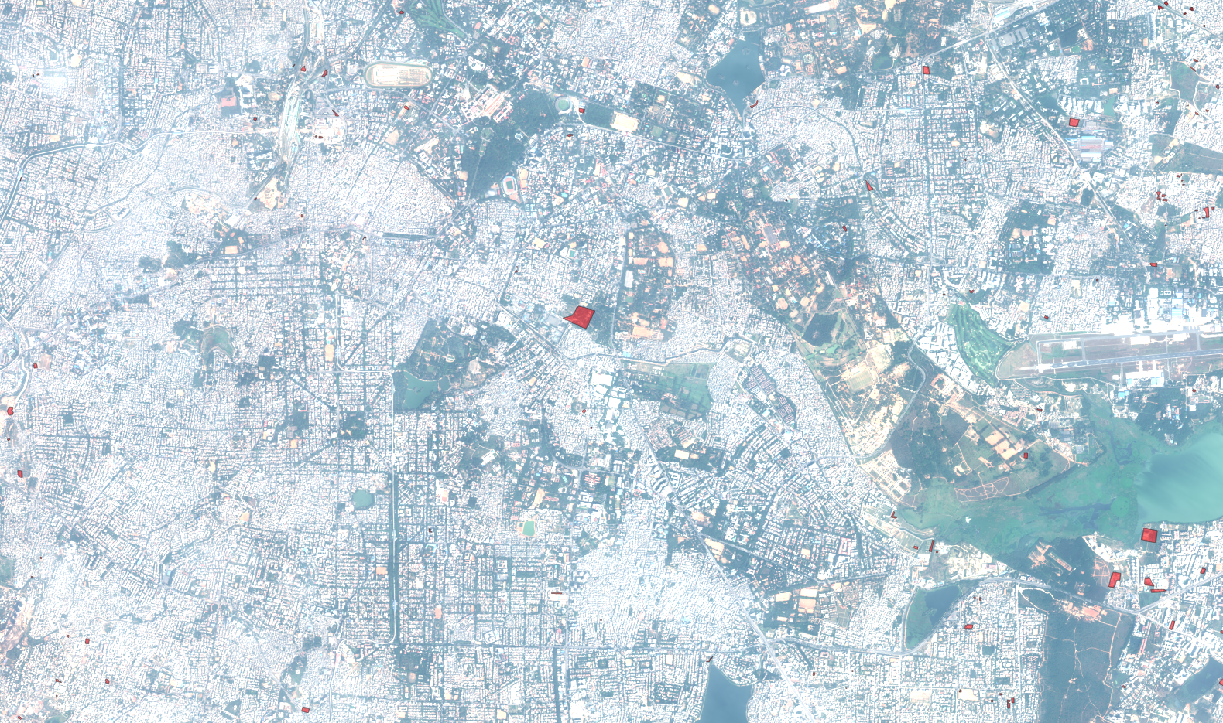
\includegraphics[width=\linewidth]{images/west-bangalore}
%  \caption{A part of western Bangalore, the red patches indicate informal
%  settlements}
%  \label{fig:west-bangalore}
%\end{figure}

\subsection{Challenges}

The distinction between formal and informal regions is often quite challenging,
in part due to the vagueness of borders between the regions. The border between
formal and informal regions often resembles more of a spectrum than a clear cut line.
Besides border difficulties, some areas are not designated as informal, while
still posessing characteristics of an informal region. This results in
a dataset with noise and inconsistency.  All in all, the binary classification
of a region encounters difficulties when applied in practice. 

Another challenge encountered in this field is the scarcity of informal
settlements.  Eventhough Banglore  has an abundance of informal settlements,
the fast majority of land is identified as formal area's. Figure
\ref{fig:sections}d shows a part of western Bangalore where it is clear
that informal settlements are sparce and distributed throughout the city. A comprehensive view of the distribution of informal settlements in this area is provided in the appendix. As
a result, the dataset of formal and informal regions becomes quite skewed.
Furthermore, because everything that is not informal is automatically
considered formal, the formal regions have a large amount of variance of visual
properties.  To illustrate: lakes, forrests, and fields fall in the same
catagory as formal residential and industrial areas while the visual
characteristics are significantly different. The diverse content of the formal
set of visual characteristics might hinder the effectiveness of differentiating
between formal and informal regions. 

To reduce the skewedness between informal and formal, only subsections of
Figure \ref{fig:west-bangalore} are used where the proportion formal to
informal is less one-sided. The sections together with their position in the whole image, are displayed in Figure \ref{fig:sections}. A smaller difference in formal informal ratio allows for
a better understanding of the effectiveness of various features. The features
are assesed using these area's 

%\begin{figure}
%\centering
%  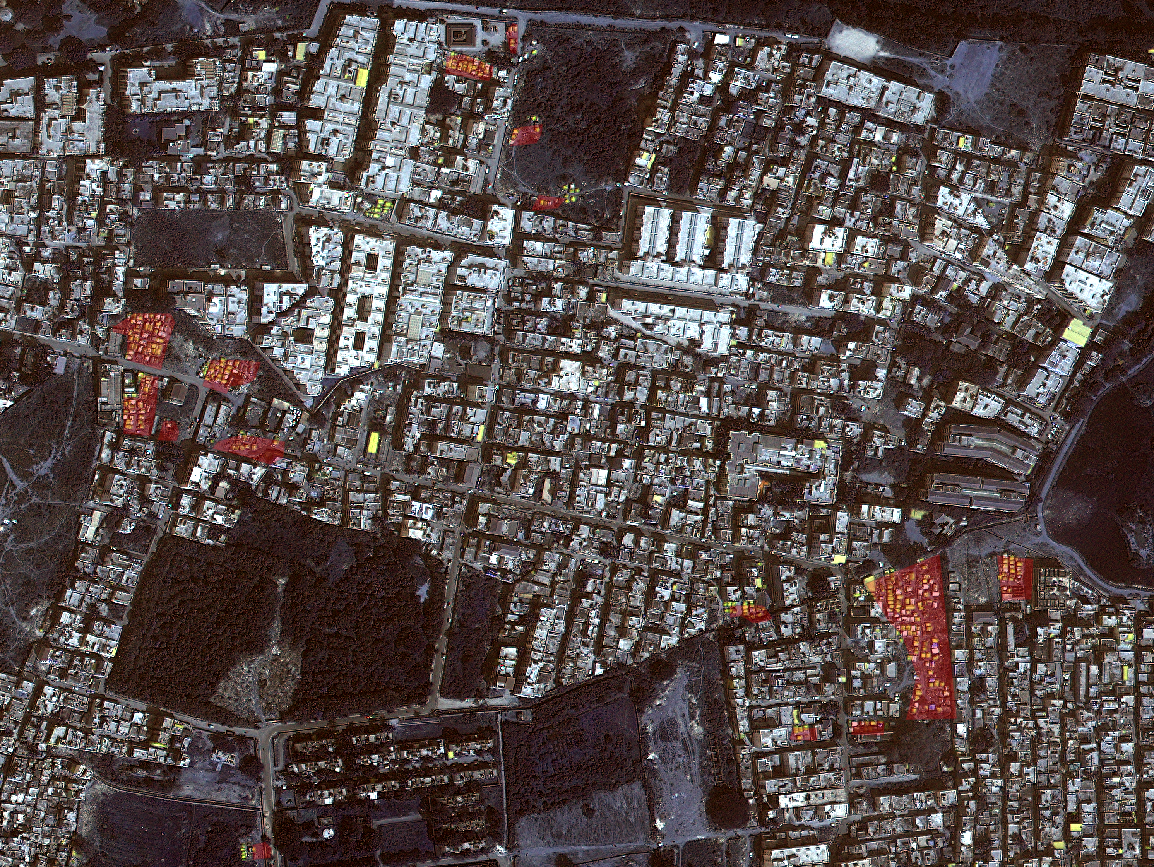
\includegraphics[width=\linewidth]{images/section_3}
%  \caption{Dense informal area in Bangalore, the red patches indicate informal
%  settlements}
%  \label{fig:section_3}
%\end{figure}


\begin{figure}
\centering
\begin{tabular}{cc}
  \subfloat[Section 1]{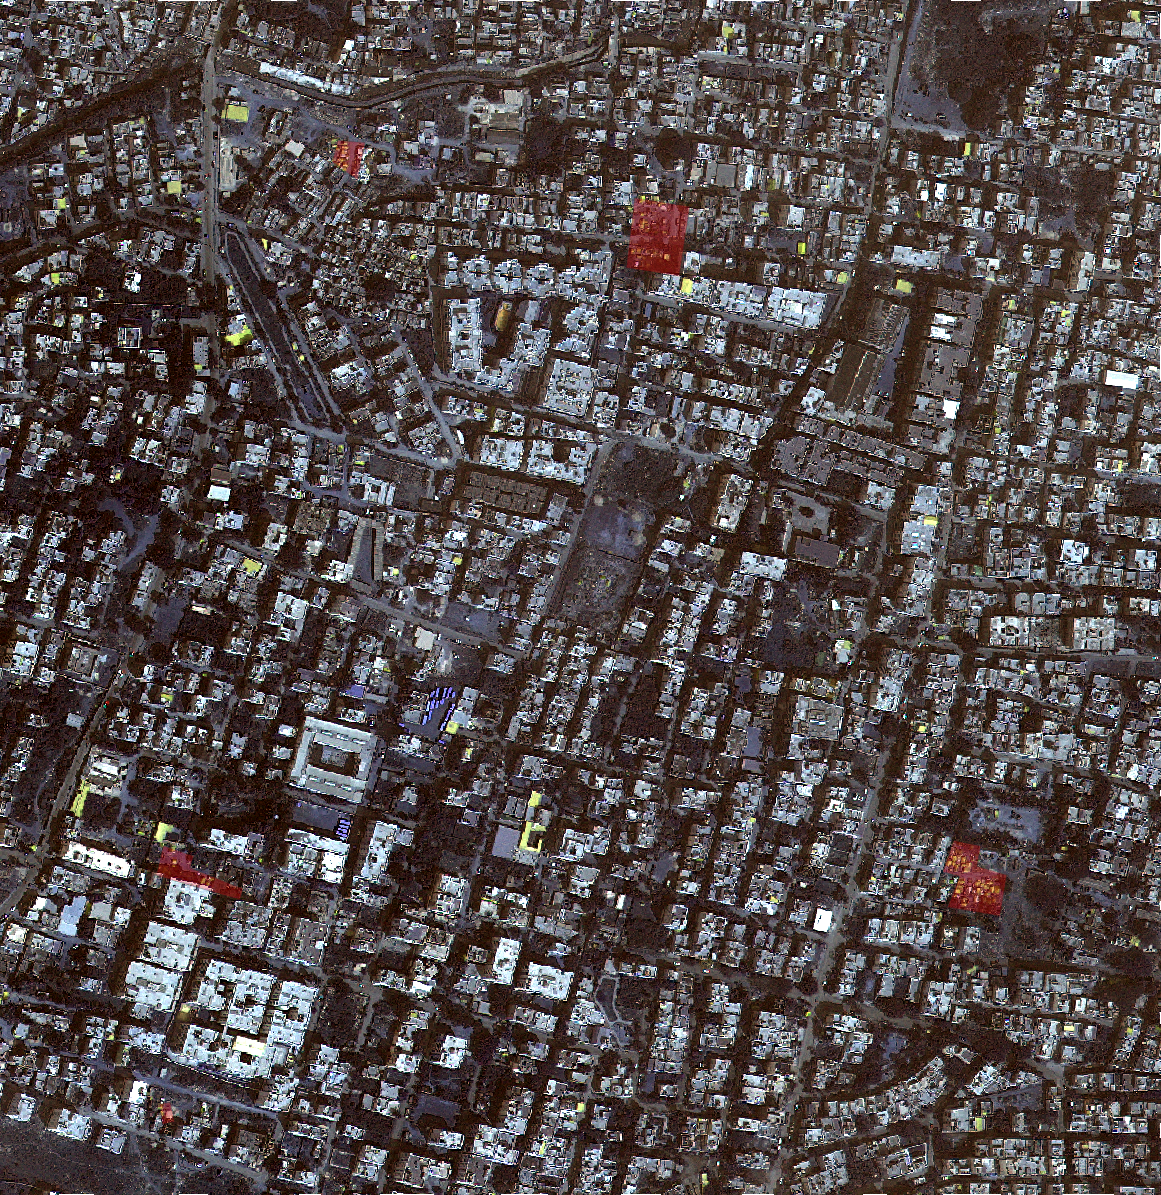
\includegraphics[width=6.2cm, height=5cm]{images/section_1}}&
  \subfloat[Section 2]{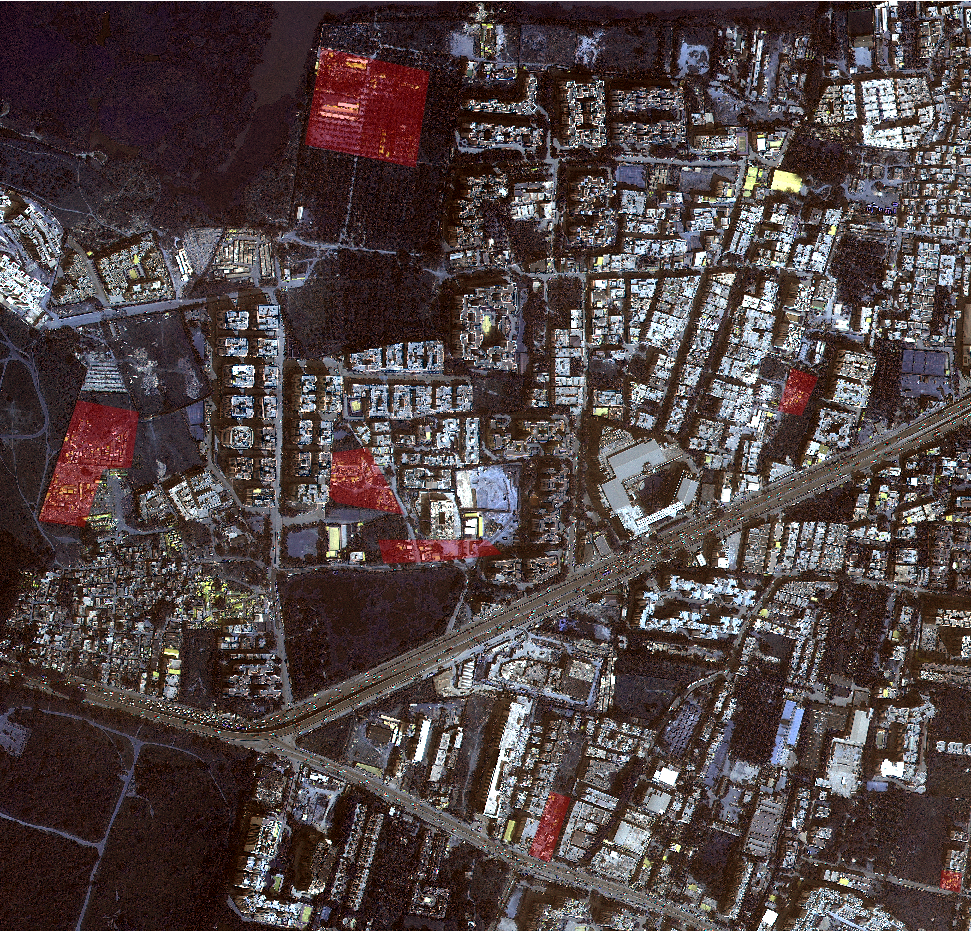
\includegraphics[width=6.2cm, height=5cm]{images/section_2}}\\
  \subfloat[Section 3]{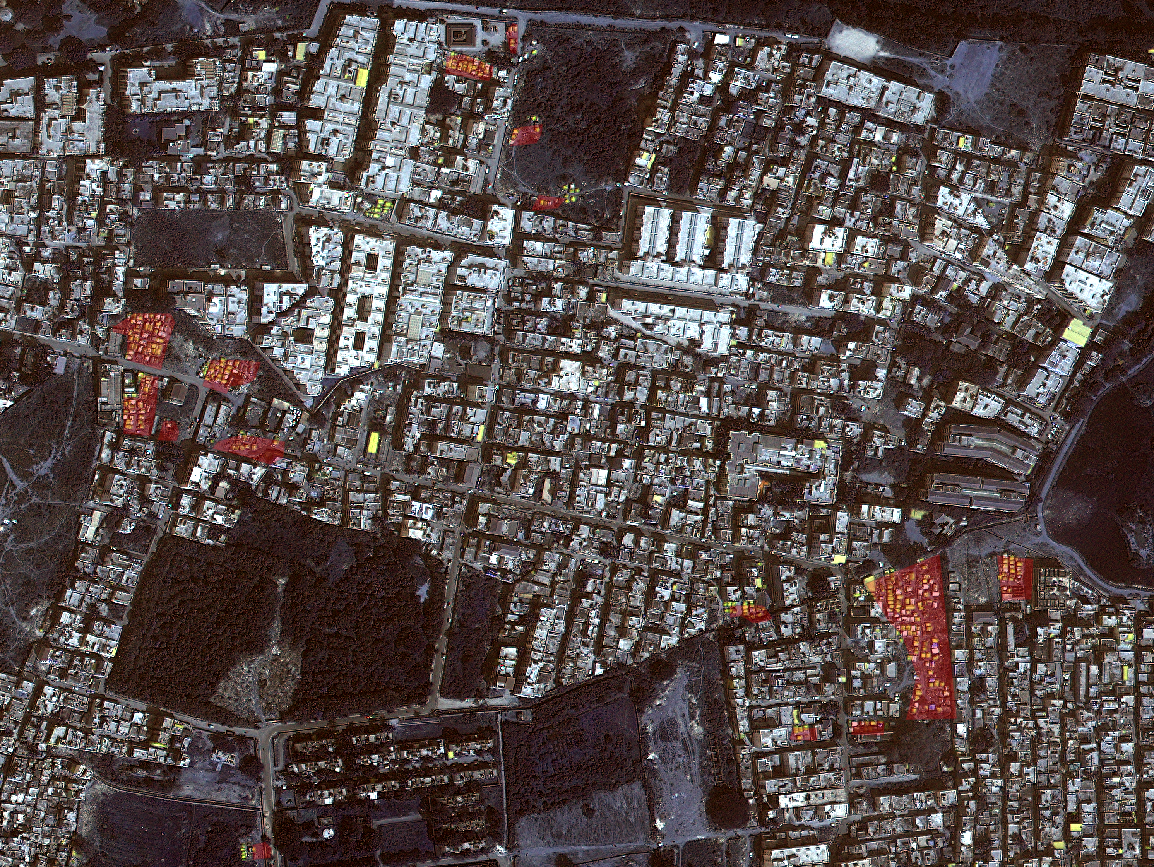
\includegraphics[width=6.2cm, height=5cm]{images/section_3}}&
  \subfloat[Location of Sections]{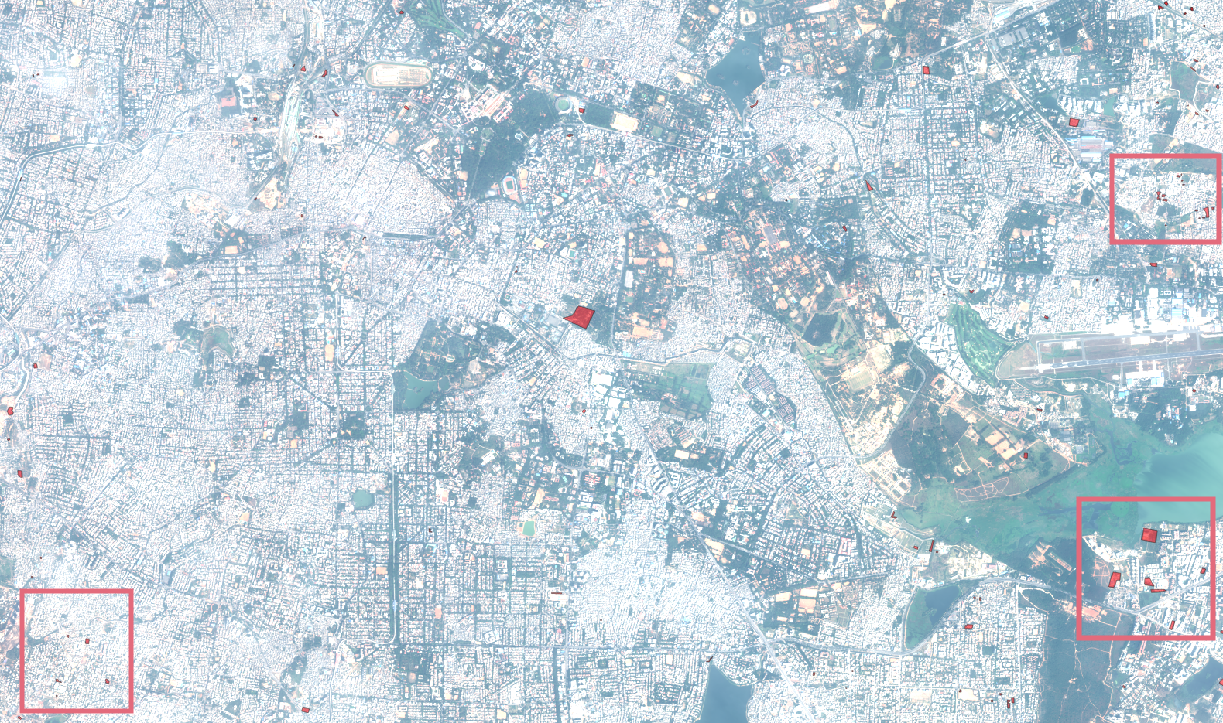
\includegraphics[width=6.2cm]{images/west-bangalore_sections}}
\end{tabular}
\caption{The images used for evaluation and classification}
\label{fig:sections}
\end{figure}

